% Chapter 3

\chapter{Implementation Details}
\label{Chapter3}
In this chapter we take a walk through the Matlab code to examine various implementation details. \refFig{workflow} diagrams an overview of workflow in \texttt{Fermium} (Finite Element Research Methods Implemented Using Matlab). As this code was developed primarily as a test-bed for various high-order finite element methods on a limited set of test problems, no effort has gone toward making a general interface to set up problems of more practical engineering interest. Also, \texttt{Fermium} was developed in Matlab as an initial prototype for a more powerful and general FEM testbed currently being developed in C++.

In order to facilitate debugging and reduce overhead and CPU time, most of the code functions as one giant script file with few actual function calls. This is done via a useful property of Matlab: the ability to embed scripts in other scripts. This allows us to minimize code redundancy while easing the job of debugging and analysis.

\newpage
\begin{textblock*}{7.5in}(.5in,1in)
\centering
   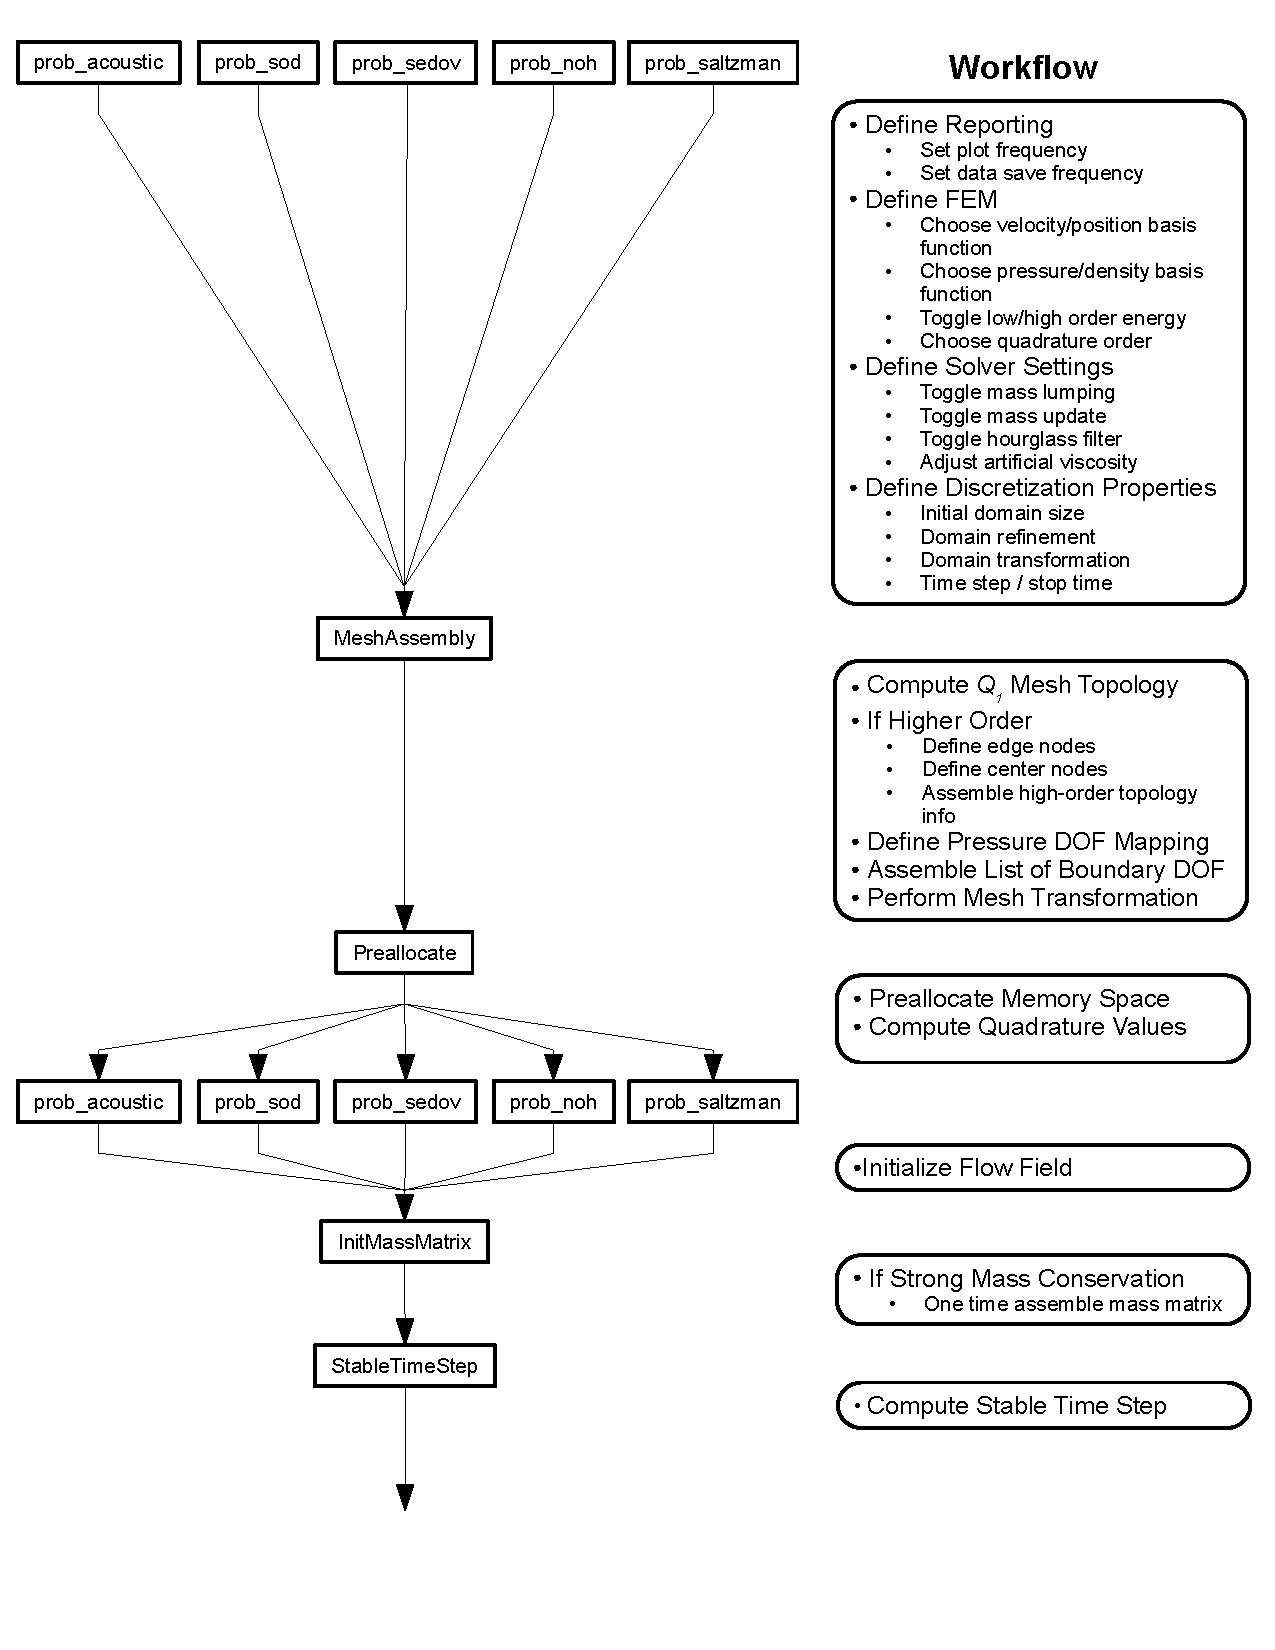
\includegraphics[trim = 0in .5in 0in 0in,clip,width=7.5in,keepaspectratio=true]{./Figures/CodeOutline.pdf}
\end{textblock*}
\mbox{}\clearpage
\newpage

\begin{figure}[p]
\begin{textblock*}{7.5in}(.5in,1in)
\centering
   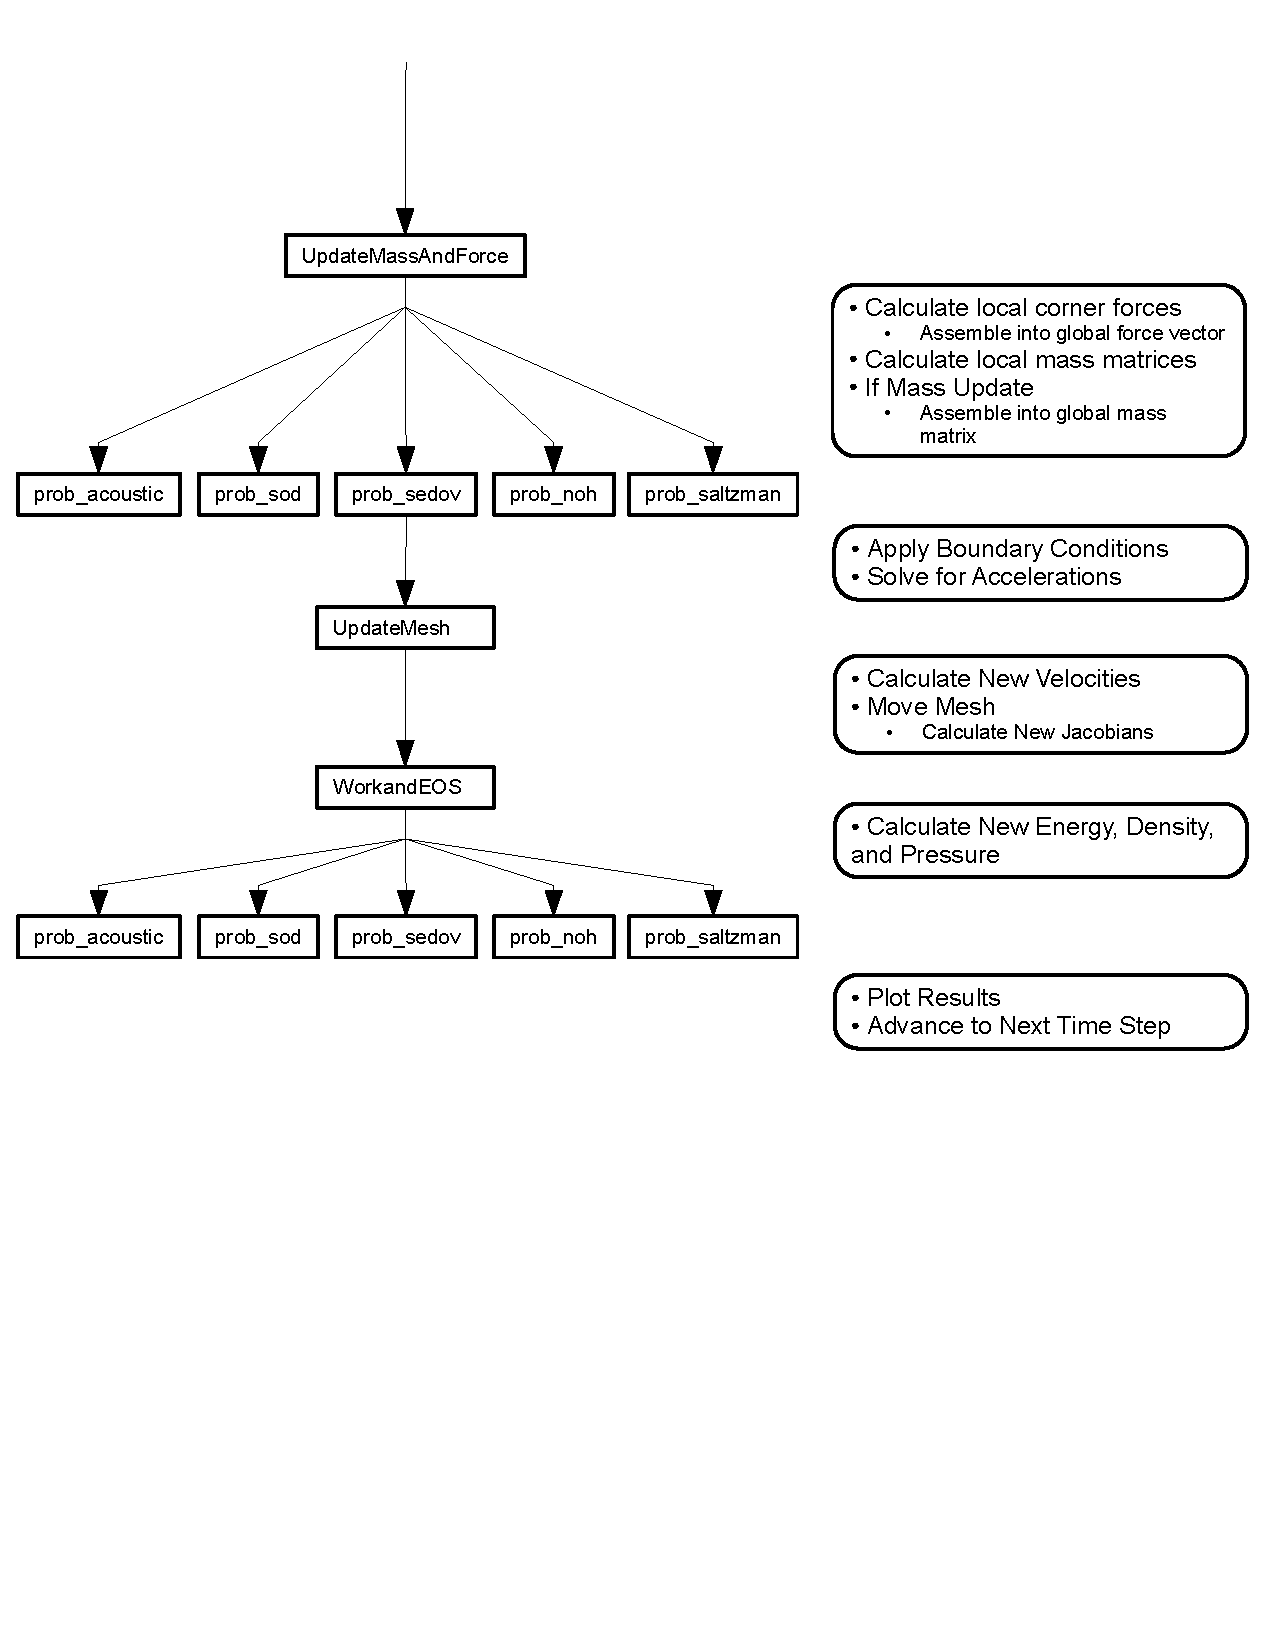
\includegraphics[trim = 0in 4in 0in 0in,clip,width=7.5in]{./Figures/CodeOutline2.pdf}
\end{textblock*}
\begin{textblock*}{3.5in}(2.5in,8in)
\caption{Workflow diagram}
 \label{fig:workflow}
\end{textblock*}
\end{figure}
\mbox{}\clearpage
\newpage

\section{The Drivers} \label{sec:strongmassupdate}
Starting at the top of the workflow diagram, we see the drivers: scripts which define a problem and connect all of the pieces necessary to solve it. We have implemented several classic test problems as drivers including the acoustic wave problem, the Sod shock tube, the Sedov explosion, the Noh implosion, the piston driven shock, and the Saltzman piston, the details of which can be found in \refChap{Elements} (acoustic wave) and \refChap{NumericalResults} (Sod, Noh, Saltzman, and Sedov).

The first thing that we need to set in our code is the method that we want to use to solve the problem. \texttt{Fermium} is general enough to allow for the kinematic and thermodynamic basis functions to be chosen independently. Hence, we have the following options available for the velocity/position basis functions: bi-linear, bi-quadratic, and bi-linear with bubble, as illustrated in \refFig{VelBasisFunctions}. All of these basis functions are defined on quadrilaterals, but there is nothing to prevent us from trying triangles or any other shape (other than the added complexity of going to unstructured grids). We have many more thermodynamic basis functions at our disposal, as depicted in \refFig{PresBasisFunctions}. At this point higher order energy is still in an experimental stage. From some initial results, it looks like we are able to achieve higher order pressure and density behavior while maintaining piecewise constant energy representations. Therefore, although we maintain a switch to use a higher-order energy representation, we usually represent energy as a $Q_0$ field.

\begin{figure}[p!]
 \centering
 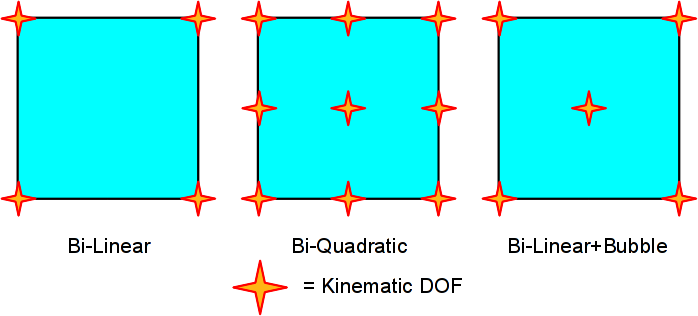
\includegraphics[width=6in,keepaspectratio=true]{./Figures/VelBasisFunctions.png}
 % VelBasisFunctions.png: 698x343 pixel, 107dpi, 16.56x8.14 cm, bb=
 \caption{Options for kinematic basis functions}
 \label{fig:VelBasisFunctions}
\end{figure}

\begin{figure}[p!]
 \centering
 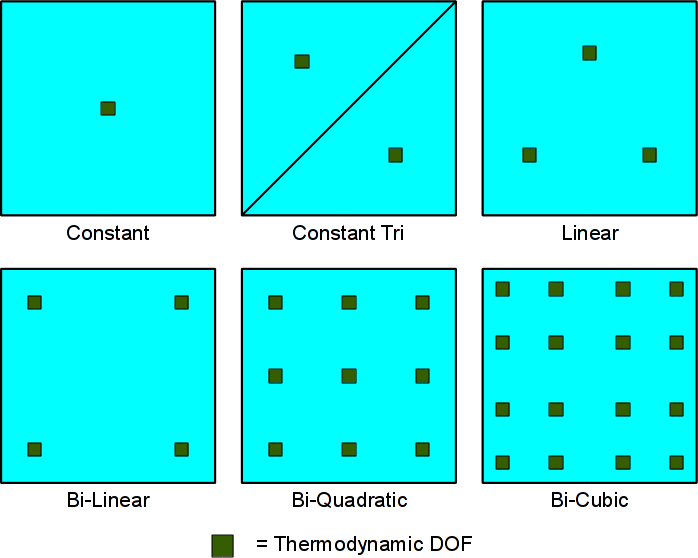
\includegraphics[width=5in,keepaspectratio=true]{./Figures/PresBasisFunctions.png}
 % VelBasisFunctions.png: 698x343 pixel, 107dpi, 16.56x8.14 cm, bb=
 \caption{Options for thermodynamic basis functions}
 \label{fig:PresBasisFunctions}
\end{figure}

Furthermore, the driver has variables to toggle several other solver options. We have derived the concept of \emph{strong mass conservation} (see \refSec{strongmass}), which allows us to avoid recomputing the mass matrix every cycle. The driver script has a switch called \texttt{MassUpdate} that allows us to forgo recalculating our mass matrix every cycle. Another consequence of strong mass conservation is that $\rho |J|=const$. Therefore, if we use $\rho |J|$ as our finite element expansion rather than $\rho$, we don't have to do a density update. The \texttt{StrongMass} switch changes the thermodynamic variables to this representation. This is also somewhat in the experimental stage, so we will mostly consider traditional finite element spaces in this research. There are also knobs to turn on and control hourglass filters and artificial viscosity. In addition to all of this, we use the driver to set the Gauss-Legendre quadrature order and the initial and maximum time steps. The mesh geometry and refinement are also controlled in the header of the driver script. We can also set plot and save-file frequency. \refTab{switches} lists the various parameters and variables that are available in the header along with a few typically used values.

\begin{table}
\centering
  \caption{List of parameters and variables}
  \label{tab:switches}
  \begin{tabular}{|l|p{2.5in}|c|}
  \hline
  Switch or Knob & Possible Values & Typical Value\\
  \hline
  \textsf{recover} & false, path to recover file &\\
  \textsf{SaveFigures} & true, false &\\
  \textsf{nplots} & $\mathbb{N} \in [0,1,2,...)$ & 20\\
  \textsf{nsaves} & $\mathbb{N} \in [0,1,2,...)$ & 10\\
  \textsf{dtInit} & $\mathbb{R} \in (0,\infty)$  & 1e-3\\
  \textsf{dtMax} &  $\mathbb{R} \in (0,\infty)$  & 1e-2\\
  \textsf{maxcycle} &  $\mathbb{N} \in [1,2,...)$ & 1e5\\
  \textsf{VBasis} & \textsf{@Q1Basis, @Q2Basis, @Q1bBasis...} & \\
  \textsf{PBasis} & \textsf{@Q0Basis, @P1Basis, @Q1dBasis...} & \\
  \textsf{HighOrderEnergy} & true, false &\\
  \textsf{StrongMass} & true, false &\\
  \textsf{FullMassMatrixSolve} & true, false &\\
  \textsf{MassUpdate} & true, false &\\
  \textsf{QuadOrder} & $\mathbb{N} \in [1,2,...)$ &\\
  \textsf{hgfrac} &  $\mathbb{R} \in [0,\infty)$ & 1 \\
  \textsf{Qfrac} &  $\mathbb{R} \in [0,\infty)$ & 1 \\
  \textsf{qquad} & $\mathbb{R} \in [0,\infty)$ & 1 \\
  \textsf{qlin} & $\mathbb{R} \in [0,\infty)$ & 1 \\
  \hline
  \end{tabular}
\end{table}

\section{Mesh Assembly and Variable Preallocation}
In the interests of code re-use, we have moved as much functionality as possible to the common files like \textsf{MeshAssembly.m} and \textsf{Preallocate.m}. The \textsf{MeshAssembly} script fleshes out the details of the FEM chosen: defining the number of spatial and thermodynamic DOFs per zone and their location within the reference element. We also need to generate a mesh and define the connectivity of the elements. The function \textsf{ComputeReferenceMeshNodes} creates a Cartesian mesh, $\mathtt{xmin} < x < \mathtt{xmax}$ by $\mathtt{ymin} < y < \mathtt{ymax}$, while \textsf{ComputeMeshTopology} defines the connectivity: which nodes belong to which quad. If the spatial discretization is higher order, we go on to further refine the mesh. If the element has additional edge nodes we place these and, along with the corner connectivity, add the edge connectivity information to \texttt{Quadmap}. Additionally, if the element has center nodes, we add this information to the end of \texttt{Quadmap}. Therefore, the velocity nodes within each element are numbered according to \refFig{VelNodeNumbering} with the corner nodes listed first and center nodes listed last. For data structure reasons, we have formulated each column of \texttt{Quadmap} as an element and each row as a spatial DOF connected to that element.

\begin{figure}[h!]
 \centering
 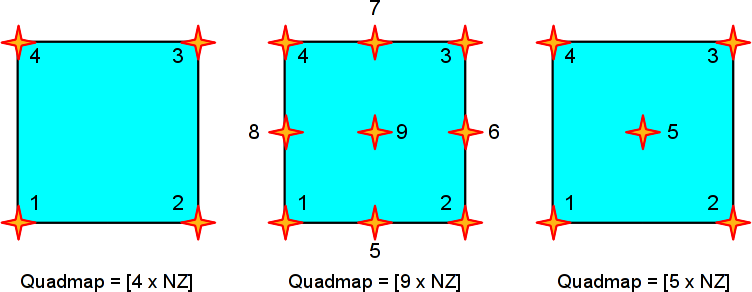
\includegraphics[width=6in,keepaspectratio=true]{./Figures/VelNodeNumbering.png}
 % VelBasisFunctions.png: 698x343 pixel, 107dpi, 16.56x8.14 cm, bb=
 \caption{Velocity node numbering}
 \label{fig:VelNodeNumbering}
\end{figure}

The pressure map is a lot simpler to set up because there is no sharing of DOFs between elements. The \texttt{PressureMap} array is as simple as \refEq{PresMap}, where each column refers to a different element and each row is a different pressure DOF belonging to that element

\newEq{PresMap}{
\mathtt{PressureMap}=\left[
\begin{array}{ccccc}
1 & npdof+1 & 2 \cdot npdof+1 & \cdots & (NZ-1)\cdot npdof+1 \\
2 & npdof+2 & 2 \cdot npdof+2 & \cdots & (NZ-1)\cdot npdof+2 \\
\vdots & \vdots & \vdots & \ddots & \vdots \\
npdof & 2 \cdot npdof & 3\cdot npdof & \cdots & NZ\cdot npdof
\end{array}\right]}

The next step is to determine which DOFs are on which boundary. This is done with the \texttt{ComputeBoundaryDOFQuad} function. \texttt{MeshAssembly} also performs any grid transformation called for by the driver, including randomly distorting the mesh, applying the Saltzman mesh pattern, rotating, or refining the mesh.

The \texttt{Preallocate} m-file mostly just preallocates empty matrices and vectors for speed (as suggested by Matlab). It also evaluates the basis functions, their derivatives, and the Jacobian at the preset quadrature points.

\section{Initializing the Flow Field}
\texttt{Preallocate.m} then returns control back to the driver where the flow field is initialized. Here the initial velocity profile and state variables are specified. After this, the \texttt{InitMassMatrix} script is called. If we are using strong mass conservation to avoid recalculating the mass matrix every cycle, this script assembles the global mass matrix which will be used for every subsequent time step. Once this is done, we go into the time stepping loop.

\section{Solving the Momentum Equation}
The first thing that we need to do at each step is to calculate a stable time increment using the \texttt{StableTimeStep} script. For traditional SGH with an explicit time-marching scheme, this typically involves the Courant–Friedrichs–Lewy \cite{CourantFriedrichsLewy28} condition. We want the time step to be such that a wave will not propagate more than the length of one cell within one time step. This can be written
\[
 \Delta t < C \frac{h}{V}
\]
where $h$ is a measure of the length across a zone, $V$ is the maximum velocity in the zone, and $C$ is typically $1/2$. For higher order elements, we must take sub-zonal physics into account. We define $h$ to be the minimum distance between any two velocity DOFs, $V$ to be the maximum velocity, and $C$ to be $1/4$, just to be safe. 
% This may be overly harsh, but it ensures a stable solution until a more detailed analysis can be performed. 
% We have not yet been able to perform a full stability analysis of high-order curvilinear finite elements, so we have chosen a very strict definition of a stable time step. 

Once we have calculated a stable time step, we dive into the \texttt{UpdateMassAndForce} script file. This script uses the current state of the pressure, velocity, and mesh to calculate forces exerted on each spatial DOF as well as the updated mass matrix (if \textsf{MassUpdate} is turned on). Let's assume for a minute that we are calculating both. To do this, we cycle through every element in the mesh and calculate a local mass matrix and `corner' force using either the \texttt{elemQ1} or \texttt{elemQ2} (this actually works for any higher order velocity basis) function. Hourglass filtering is the only real difference between these two functions. We are still using a very primitive form of an hourglass filter for higher-order elements, so we are handling the $Q_1$ elements, with their well-developed hourglass functions separately. The current $Q_2$ ``hourglass filter'' is not really an hourglass filter, per se. Instead we use a fraction of the linear term of the artificial viscosity. This serves to smooth out high frequency velocity modes, be they physical or not. This is not an acceptable course for a full hydrocode, but we are developing appropriate high order filters. The first step in the \texttt{elem*} functions is to calculate a local mass matrix from the spatial degrees of freedom. After this, we build up the corner forces with contributions from pressure gradients, artificial viscosity, and hourglass forces as described in \refChap{Theory}. 

Once these corner forces and local mass matrices are assembled into the global system via the connectivity information, control is returned to the driver where the boundary conditions are applied and the global systems $\mathbf{M}\vec{a}_x=\vec{F}_x$ and $\mathbf{M}\vec{a}_y=\vec{F}_y$ are solved for the accelerations. This can be done via mass lumping, which accumulates all off-diagonal information to the diagonal of the matrix or a full mass matrix solve. 
% If we are using strong mass conservation and the initial mesh is Cartesian, the full mass matrix will already be diagonal for every time step, which will be the case for all most test cases that we will consider. 

\section{Mesh Movement and Thermodynamic \mbox{Update}}
Once the nodal accelerations have been solved for, the driver gives control to the \texttt{UpdateMesh} common script. This script first accelerates the velocity DOFs according to \refEq{velUpdate}, then it applies any source terms to the velocity before moving the mesh nodes according to \refEq{meshUpdate}.
\newEq{velUpdate}{
\mathsf{NEWvelocity=OLDvelocity+dt*acceleration}
}
\newEq{meshUpdate}{
\mathsf{allnodes=allnodes+dt*NEWvelocity}
}
\texttt{UpdateMesh} then calculates the new Jacobian matrix for every element at every quadrature point for use in the next time step. Finally, it checks for any points where the determinant of the Jacobian is zero or negative, which would indicate that the solution has gone unstable.

Now that we have a new mesh geometry, we can calculate the new thermodynamic properties on this updated mesh using \texttt{WorkandEOS}. Please note that the thermodynamic properties are discontinuous between zones, this allows us to loop over ever element and calculate the new state independent of all other zones without assembling any sort of global system. Thus for each zone, we first calculate the change in internal energy with the dot product of the velocity DOFs and corner forces. We then proceed to the density update. As mentioned previously in \refSec{strongmassupdate}, if we use the basis functions to represent $\rho |J|$ rather than just $\rho$, this function is constant and no density update is required. However, if we are using a traditional representation of density, then we need to compute new density DOFs. The first step is analogous to assembling a local mass matrix, but instead of using the spatial basis functions, we use the density basis functions. We then solve a small $\mathtt{npdof} \times \mathtt{npdof}$ system of equations for the new density degrees of freedom as explained in \refSec{densityupdateeq}. Now that we have the energy and density, we can update the pressure point-wise according to the equation of state.

\section{Plotting}
Finally, now that all variables have been updated for the next time step, we can move back to the driver for the plotting stage. We first check that this is one of the desired plot or save time steps. We have developed several finite element specific plotting routines such as \texttt{PlotFEMContourf} and \texttt{PlotFEMMesh} to accurately represent any arbitrary basis function to any user-specified precision. The driver plots the fields as called for, saves the figures / variable data if requested, then loops back to \texttt{StableTimeStep} for the next time step. This whole process repeats until \textsf{tstop} is reached or \texttt{WorkandEOS} detects that the solution has gone unstable.